\chapter{Diagramme entités-associations}

\section{Diagramme}

\begin{figure}
  \centering
  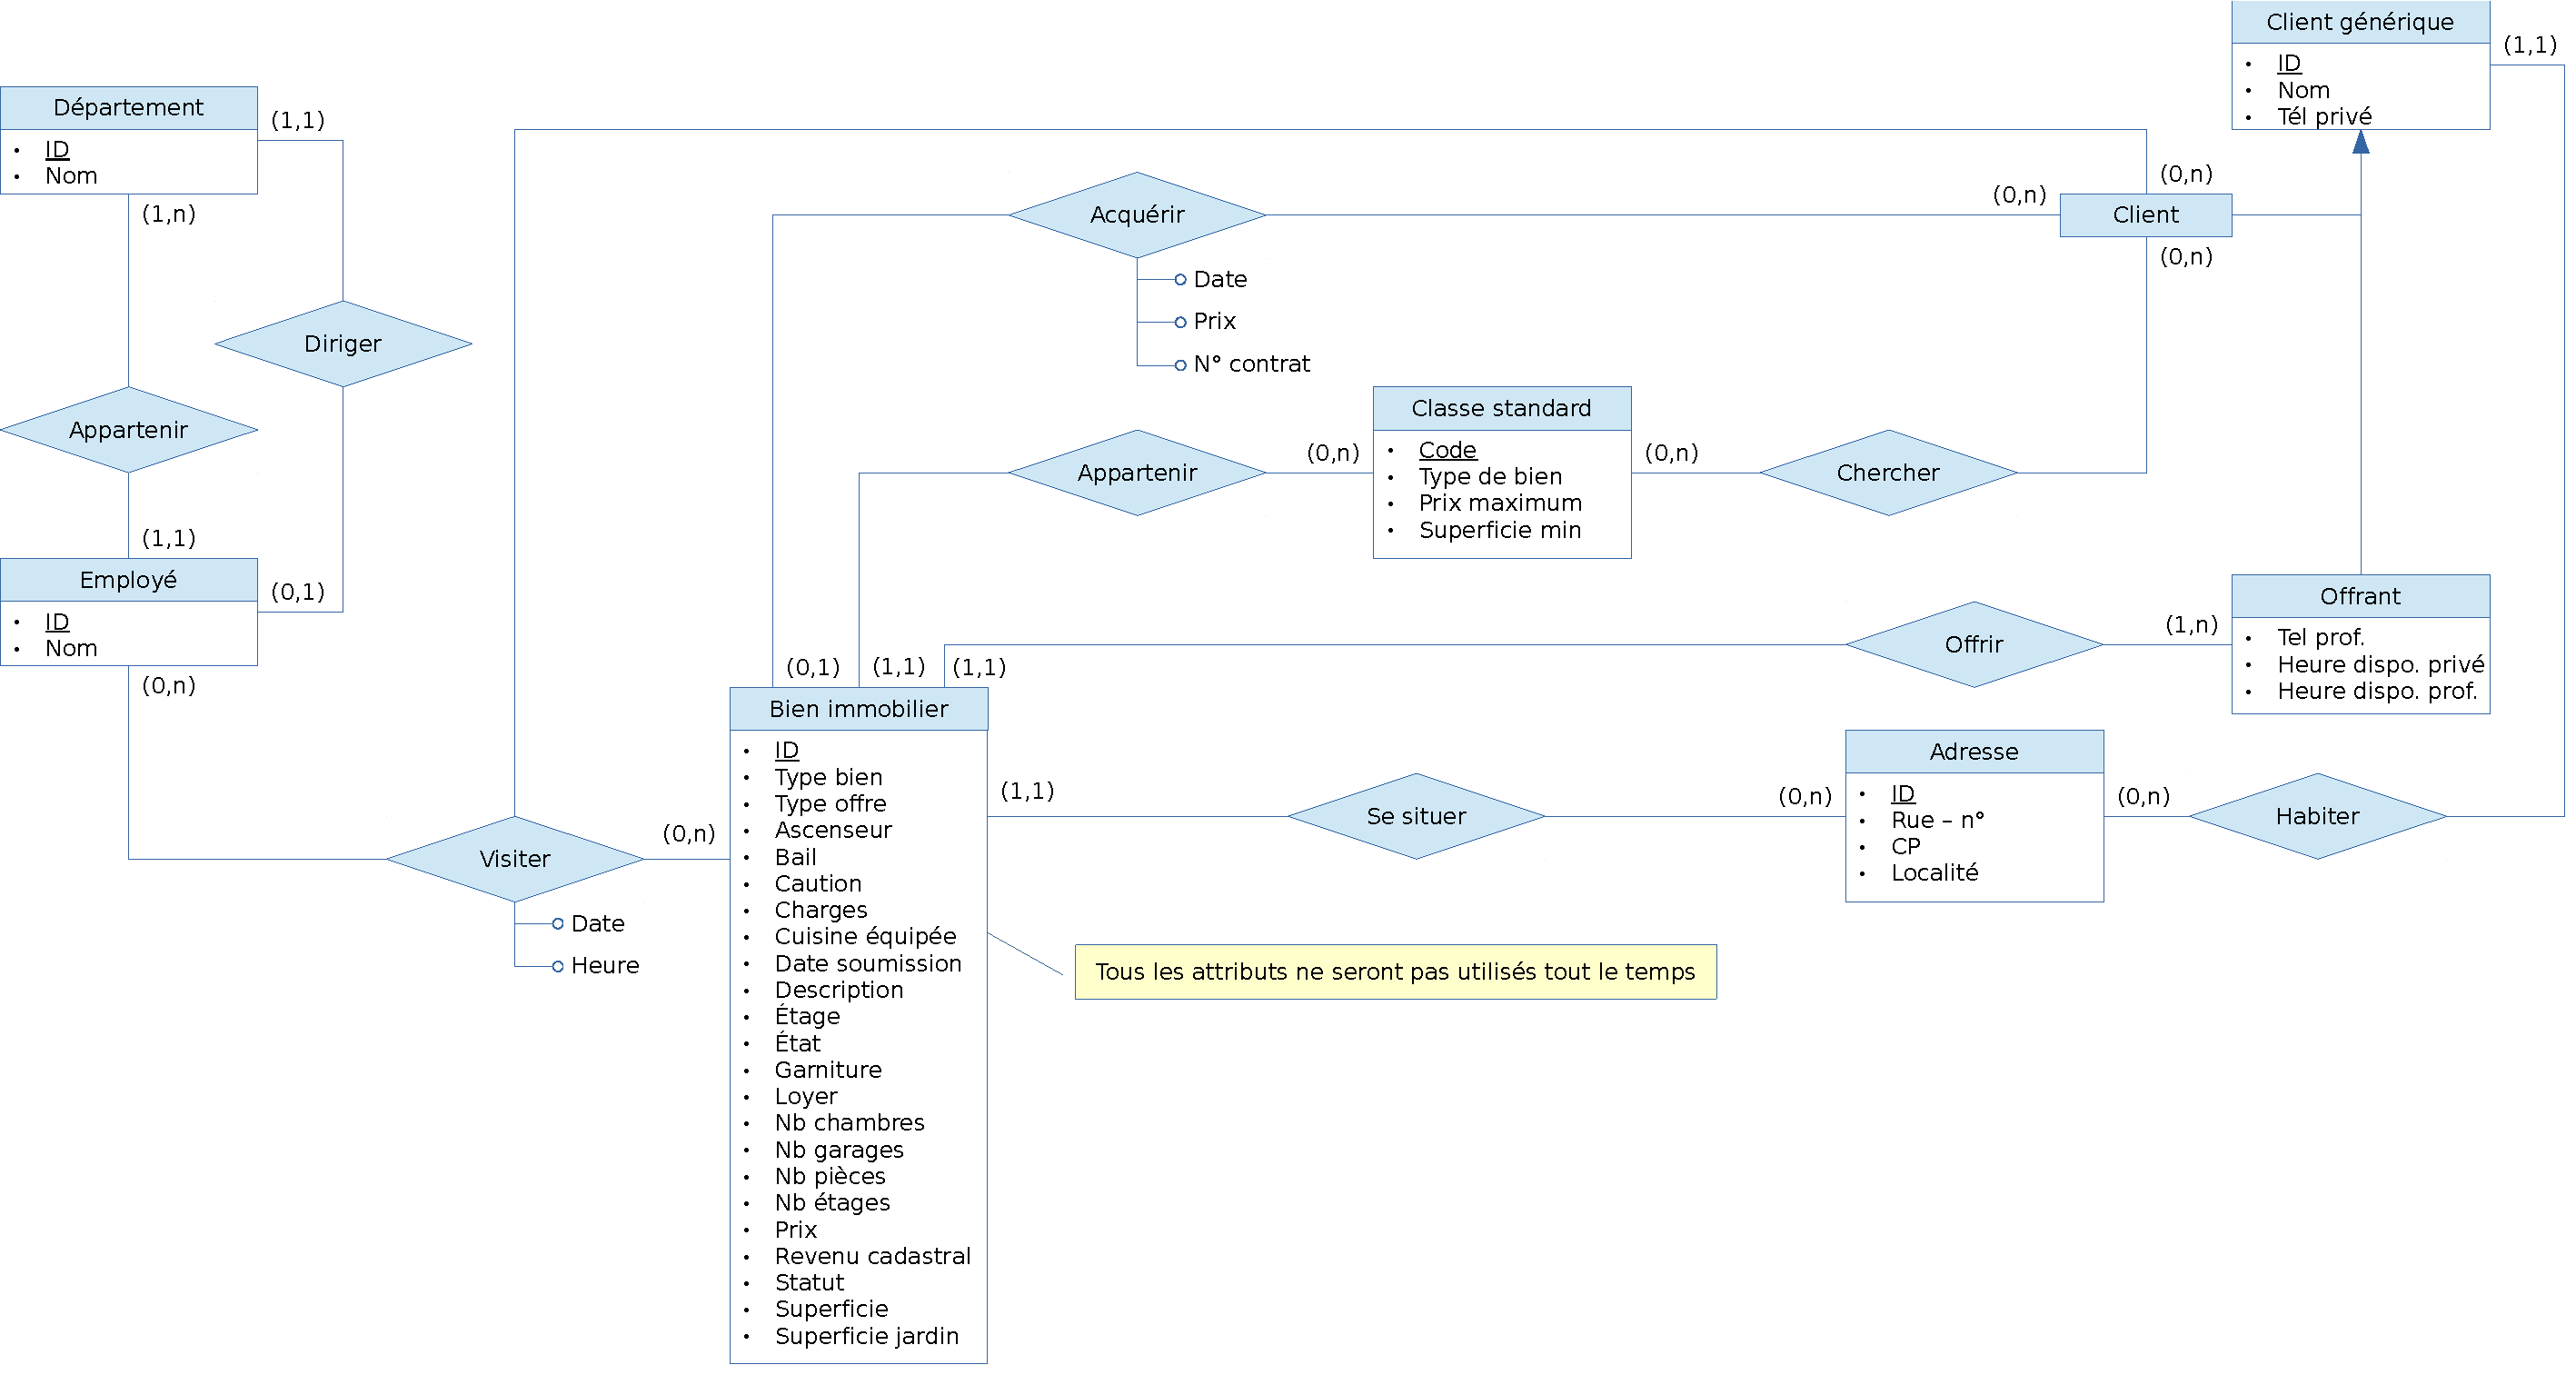
\includegraphics[angle=90,height=0.95\textheight]{IMG/er}
  \caption{Diagramme entités-associations}
  \label{img_er}
\end{figure}

La figure \refpage{img_er} illustre les entités du projet et leurs association.

\section{Rapport}

J'ai réalisé ce diagramme en deuxième lieu afin d'avoir une vue globale de l'organisation des données sur lesquelles je vais travailler.

Vu la complexité des biens immobiliers, j'ai décidé d'utiliser le concept de décorateurs (\emph{Decorator pattern}) des patrons de conception (\emph{design pattern})\footnote{Cf. \url{http://design-patterns.fr/decorateur}}. J'ai défini une entité générale pour les biens immobiliers. Ensuite, j'ai défini une hiérarchie d'entités contenant des attributs communs ou reprenant des concepts déclarés. Ainsi, l'entité \og{}Appartement\fg{} n'a pas d'attributs propre, mais c'est un concept en soi. Pour les attributs pouvant se trouver dans différentes entités, j'ai défini des décorateurs, comme par exemple pour les biens à louer.

J'ai défini une entité \og{}Adresse\fg{} qui sera associée aussi bien aux clients qu'au biens immobiliers. En effet, le concept de localisation des biens immobiliers est identique à celui de localisation des clients.

J'ai défini une entité générique pour les client. Ensuite j'ai créé des entités plus spécialisées pour les clients offrants et les clients cherchant un bien. À mon sens, un client qui aujourd'hui est un client cherchant un bien peut demain être un client offrant un bien, d'où l'utilisation d'un client générique. L'entité \og{}Client\fg{} n'offre actuellement pas d'attributs supplémentaires par rapport au client générique. J'ai quand-même créé une entité spécialisée pour permettre une éventuelle évolution future.